\documentclass[12pt]{article}
\usepackage[dvipsnames]{xcolor}
\usepackage[english]{babel}
\usepackage[utf8]{inputenc}
\usepackage{fancyhdr}
\usepackage{tikz}
\usepackage{amsmath}
\usepackage{float}
\usetikzlibrary{angles,quotes}
\usetikzlibrary{calc}
\usepackage[font=small,labelfont=bf]{caption}

\begin{document}

\begin{titlepage}
    \begin{center}
        \vspace*{1cm}
        \textbf{Head to Tail Method of Vector Addition}

        \vspace{0.5cm}
        Lab: 01

        \vspace{1cm}

        \textbf{Jaden Moore}

        \vfill

        Orange Coast College\\
        Physics A185L\\
        August 30th, 2020

    \end{center}
\end{titlepage}

\pagestyle{fancy}
\fancyhf{}
\setlength{\headheight}{15pt}
\lhead{Head to Tail Method of Vector Addition}
\rhead{Lab: 01}
\cfoot{\thepage}

\section{Introduction}

In the natural world and in the exploration of physical phenomena, it is often the case that a multitude of different forces can be acting on a single particle at any given time.

Forces acting on a particle are often represented as \textbf{vectors}. This is because a vector is a quantity that maintains both a magnitude and a direction, which can be viewed as a force in the real world. We can represent the sum of all vectors acting on a particle as a single vector known as the \textbf{resultant vector}. The resultant vector is the result of adding all vector forces acting on a particle into one single vector. In this lab, we will discuss two different methods of adding vectors and determine whether both methods are able to arrive at similar results. The methods we will discuss are known as the \textbf{head to tail method} and the \textbf{component method}. I hypothesize that both methods will yeild similar results but the head to tail method will be slightly less accurate due to the limitations in the precision of physical tools.

\section{The Head to Tail Method}
The Head to Tail method, or the visual method of vector addition, requires a precise drawing of the vectors on some x-y coordinate plane, where the head of one vector is aligned to the tail of another vector until all the vectors are orientated in a manner in which a new vector can be drawn from the tail of the first vector to the head of the last vector.

Consider a particle centered at the origin with forces acting as such:

\begin{figure}[H]
    \centering

    \caption[10pt]{A particle whose forces acting upon it are angled in arbitrary directions.}

    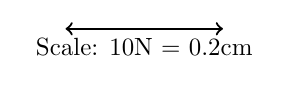
\begin{tikzpicture}[scale=0.2, every node/.style={scale=0.9}]
        \draw[thick, <->] (-5cm,0) -- node[below] {Scale: 10N = 0.2cm} (5cm,0);
    \end{tikzpicture}

    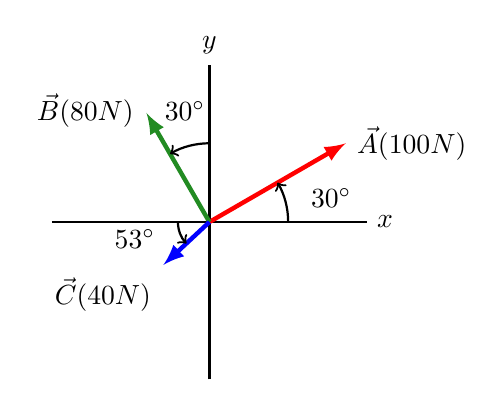
\begin{tikzpicture}[scale=0.2]

        \coordinate (O) at (0,0);

        \draw[thick, -] (-10cm,0cm) coordinate(leftx) -- (10cm,0cm) coordinate(rightx) node[right,fill=white]{$x$};

        \draw[thick, -] (0cm,-10cm) coordinate(bottomy) -- (0cm,10cm) coordinate(topy) node[above,fill=white] {$y$};

        \draw[red, ultra thick, -latex] (0cm,0cm) -- (30:10cm) coordinate(A) node[pos=1,anchor=west, black]{$\vec{A} (100 N)$};

        \draw[ForestGreen, ultra thick, -latex] (0cm,0cm) -- (120:8cm) coordinate(B) node[pos=1.02,anchor=east, black]{$\vec{B} (80 N)$};

        \draw[blue, ultra thick, -latex] (0cm,0cm) -- (223:4cm) coordinate(C) node[pos=1.02,anchor=north east, black]{$\vec{C} (40 N)$};

        \pic [draw, ->, "$30^\circ$", angle eccentricity=1.2, anchor=west, thick, angle radius=1cm] {angle = rightx--O--A};

        \pic [draw, ->, "$30^\circ$", angle eccentricity=1.2, anchor=south, thick, angle radius=1cm] {angle = topy--O--B};

        \pic [draw, ->, "$53^\circ$", angle eccentricity=1.5, anchor=east, thick, angle radius=0.4cm] {angle = leftx--O--C};

    \end{tikzpicture}
\end{figure}

Using the Head to tail method, we can reconfigure the graph such that the heads of the vectors act as the starting point for the tail of the following vector. This can be seen as \textbf{translating} the vectors in a way where the resultant vector becomes obvious:

\begin{figure}[h]
    \centering

    \caption{A particle centered at (0,0) with the forces acting upon it arranged from head to tail.}

    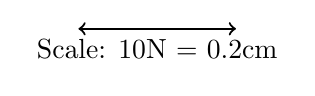
\begin{tikzpicture}[scale=0.2]
        \draw[thick, <->] (-10cm,0) -- node[below] {Scale: 10N = 0.2cm} ++(10cm,0);
    \end{tikzpicture}

    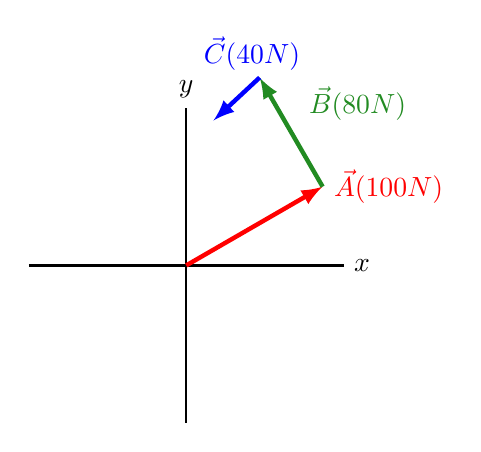
\begin{tikzpicture}[scale=0.2]

        \coordinate (O) at (0,0);

        \draw[thick, -] (-10cm,0cm) coordinate(leftx) -- (10cm,0cm) coordinate(rightx) node[right,fill=white]{$x$};

        \draw[thick, -] (0cm,-10cm) coordinate(bottomy) -- (0cm,10cm) coordinate(topy) node[above,fill=white] {$y$};

        \draw[red, ultra thick, -latex] (0cm,0cm) -- (8.66cm, 5cm) coordinate(A) node[pos=1,anchor=west, red]{$\vec{A} (100 N)$};

        \draw[ForestGreen, ultra thick, -latex] (8.66cm, 5cm) -- ($ (A) + (-4cm,6.93cm) $) coordinate(B) node[pos=1.02,anchor=north west , shift={(0.5, 0)}, ForestGreen]{$\vec{B} (80 N)$};

        \draw[blue, ultra thick, -latex] ($ (A) + (-4cm,6.93cm) $) -- ($ (B) + (-2.93cm, -2.73cm) $) coordinate(C) node[pos=1.02,anchor=south, shift={(0.5, 0.5)}, blue]{$\vec{C} (40 N)$};

    \end{tikzpicture}

\end{figure}

In this case, the resultant vector can easily be drawn by drawing a new vector $\vec{R}$ starting at the position of the first vector $\vec{A}$ and ending at the head of the last vector $\vec{C}$.

\begin{figure}[H]
    \centering
    \caption{A particle centered at (0,0) whose forces can all be summed up into a single vector $\vec{R}$.}

    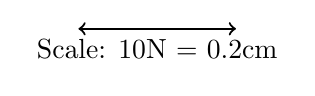
\begin{tikzpicture}[scale=0.2]
        \draw[thick, <->] (-10cm,0) -- node[below] {Scale: 10N = 0.2cm} ++(10cm,0);
    \end{tikzpicture}

    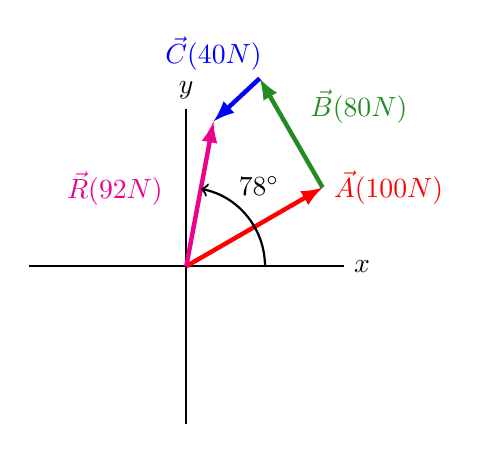
\begin{tikzpicture}[scale=0.2]

        \coordinate (O) at (0,0);

        \draw[thick, -] (-10cm,0cm) coordinate(leftx) -- (10cm,0cm) coordinate(rightx) node[right,fill=white]{$x$};

        \draw[thick, -] (0cm,-10cm) coordinate(bottomy) -- (0cm,10cm) coordinate(topy) node[above,fill=white] {$y$};

        \draw[red, ultra thick, -latex] (0cm,0cm) -- (8.66cm, 5cm) coordinate(A) node[pos=1,anchor=west, red]{$\vec{A} (100 N)$};

        \draw[ForestGreen, ultra thick, -latex] (8.66cm, 5cm) -- ($ (A) + (-4cm,6.93cm) $) coordinate(B) node[pos=1, anchor=north west, shift={(0.5, 0)}, ForestGreen]{$\vec{B} (80 N)$};

        \draw[blue, ultra thick, -latex] ($ (A) + (-4cm,6.93cm) $) -- ($ (B) + (-2.93cm, -2.73cm) $) coordinate(C) node[pos=1,anchor=south, shift={(0, 0.5)}, blue]{$\vec{C} (40 N)$};

        \draw[magenta, ultra thick, -latex] (0cm,0cm) -- ($ (B) + (-2.93cm, -2.73cm) $) coordinate(R) node[shift={(-0.5, -0.5)}, pos=1,anchor=north east, magenta]{$\vec{R} (92 N)$};

        \pic [draw, ->, "$78^\circ$", angle eccentricity=1.2, anchor=south, thick, angle radius=1cm] {angle = rightx--O--R};

    \end{tikzpicture}
\end{figure}

In this case, the vector $\vec{R}$ is equal to the sum of $\vec{A}$, $\vec{B}$, $\vec{C}$. That is:

\[\vec{A} + \vec{B} + \vec{C} = \vec{R}\]

Calculating the approximate magnitude and direction of vector $\vec{R}$, graphically, requires the use of a few precise measuring instruments such as a protractor and straight-edge ruler which has been done in the attached hand drawings. Given a scale of 10N = 1cm, I arranged the given vectors from head to tail using a protractor and ruler. I then approximated the magnitude of vector $\vec{R}$ by measuring the distance between the start of vector $\vec{A}$ to the head of vector $\vec{C}$ which equated to approximately 9.2cm, or 92 Newtons. The direction of vector $\vec{R}$ was approximated with the use of a protractor centered at (0,0) which equated to approximately \(78.0^\circ{}\) starting from the positve x-axis. Now we will be able to compare these results with the following method and examine any diffferences in the result.

\section{The Vector Component Method}
A more precise method of calculating the sum of multiple vectors is using the \textbf{Vector Component Method}. The component method involves calculating the length of the projection of each vector onto the x and y axis and then summing the individual projections. The result being a single set of vector components that represent the components of the resultant vector $\vec{R}$.

Consider the same vectors we discussed in the Head to Tail experiment but this time we will approach it from the component method:

\begin{figure}[H]
    \caption{The original graph from Figure 1.}
    \centering
    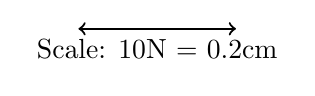
\begin{tikzpicture}[scale=0.2]
        \draw[thick, <->] (-10cm,0) -- node[below] {Scale: 10N = 0.2cm} ++(10cm,0);
    \end{tikzpicture}

    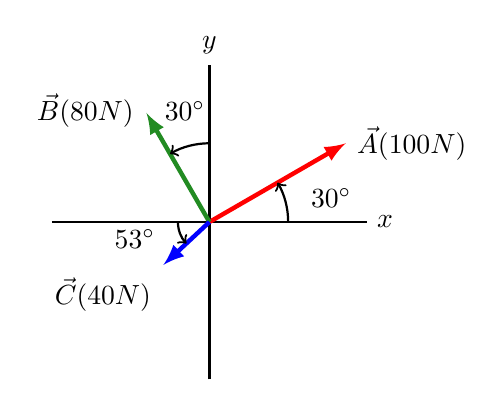
\begin{tikzpicture}[scale=0.2]

        \coordinate (O) at (0,0);

        \draw[thick, -] (-10cm,0cm) coordinate(leftx) -- (10cm,0cm) coordinate(rightx) node[right,fill=white]{$x$};

        \draw[thick, -] (0cm,-10cm) coordinate(bottomy) -- (0cm,10cm) coordinate(topy) node[above,fill=white] {$y$};

        \draw[red, ultra thick, -latex] (0cm,0cm) -- (30:10cm) coordinate(A) node[pos=1,anchor=west, black]{$\vec{A} (100 N)$};

        \draw[ForestGreen, ultra thick, -latex] (0cm,0cm) -- (120:8cm) coordinate(B) node[pos=1.02,anchor=east, black]{$\vec{B} (80 N)$};

        \draw[blue, ultra thick, -latex] (0cm,0cm) -- (223:4cm) coordinate(C) node[pos=1.02,anchor=north east, black]{$\vec{C} (40 N)$};

        \pic [draw, ->, "$30^\circ$", angle eccentricity=1.2, anchor=west, thick, angle radius=1cm] {angle = rightx--O--A};

        \pic [draw, ->, "$30^\circ$", angle eccentricity=1.2, anchor=south, thick, angle radius=1cm] {angle = topy--O--B};

        \pic [draw, ->, "$53^\circ$", angle eccentricity=1.5, anchor=east, thick, angle radius=0.4cm] {angle = leftx--O--C};

    \end{tikzpicture}
\end{figure}

\paragraph{}

We calculate the x component of any vector $\vec{V}$ by multiplying its magnitude by the cosine of the angle $\theta$ that it makes with respect to the positive x-axis:

\[ \vec{V_x}= |\vec{V}|\cos{\theta}\]

and similarly the y-component:

\[\vec{V_y}= |\vec{V}|\sin{\theta}\]

From this, we are able to derive the components of the resultant vector $\vec{R}$ by summing the components of each individual vector from the graph. That is:

\[\vec{R_x}= \vec{A_x} + \vec{B_x} + \vec{C_x} \]
and
\[\vec{R_y}= \vec{A_y} + \vec{B_y} + \vec{C_y}\]

Consider the following table which demonstrates the process of vector componenet addition:

\paragraph{}

\setlength{\tabcolsep}{18pt}
\renewcommand{\arraystretch}{1.5}

\begin{figure}[H]
    \centering
    \begin{tabular}{ |p{3cm}|p{3cm}|p{3cm}| }
        \hline
        \multicolumn{3}{|c|}{Table 1: The addition of the vector components}  \\
        \hline
        Vector $\vec{V}$                  & $\vec{V_x}$ (N) & $\vec{V_y}$ (N) \\
        \hline
        $\vec{A}$                         & 86.6            & 50.0            \\
        $\vec{B}$                         & -40             & 69.3            \\
        $\vec{C}$                         & -29.3           & -27.3           \\
        \hline
        $\vec{A}$ + $\vec{B}$ + $\vec{C}$ & 17.3            & 92.0            \\
        \hline
    \end{tabular}
\end{figure}

\paragraph{}

In this case, let $\vec{R}$ = $\vec{A}$ + $\vec{B}$ + $\vec{C}$ whose vector components are $\vec{R_x}$ = 17.3N and $\vec{R_y}$ = 92.0N, which were obtained by summing the individual components of the original vectors. Now that we have the x and y components of the resultant vector, we can calculate it's magnitude and direction.

\paragraph{}

To calculate the direction of the resultant vector $\vec{R}$, we can find the angle that the resultant vector makes with respect to the x axis:

\[Let \thickspace \theta = \tan^{-1}\frac{92.0N}{17.3N} = 79.3^\circ\]

To calculate the magnitude of the vector $\vec{R}$, we can use Pythagorean's Theorum since the vector creates a right triangle with the x-axis when drawn on a coordinate plan:

\[Let \thickspace |\vec{R}|= \sqrt{(17.3N)^2 + (92.0N)^2}=93.6N\]

\paragraph{}

Thus, The resultant vector $\vec{R}$ is:

\begin{figure}[H]
    \centering

    \caption{the vector $\vec{R}$ obtained from $\vec{A}$ + $\vec{B}$ + $\vec{C}$}

    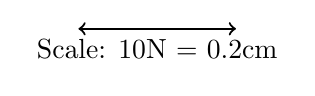
\begin{tikzpicture}[scale=0.2]
        \draw[thick, <->] (-10cm,0) -- node[below] {Scale: 10N = 0.2cm} ++(10cm,0);
    \end{tikzpicture}


    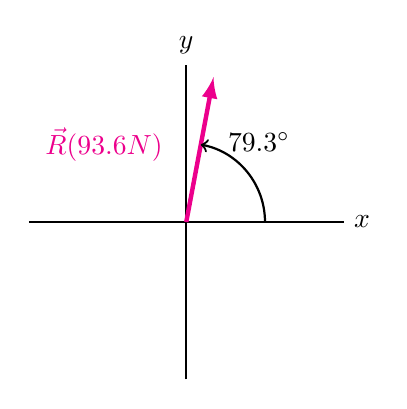
\begin{tikzpicture}[scale=0.2]

        \coordinate (O) at (0,0);

        \draw[thick, -] (-10cm,0cm) coordinate(leftx) -- (10cm,0cm) coordinate(rightx) node[right,fill=white]{$x$};

        \draw[thick, -] (0cm,-10cm) coordinate(bottomy) -- (0cm,10cm) coordinate(topy) node[above,fill=white] {$y$};

        \draw[magenta, ultra thick, -latex] (0cm,0cm) -- (1.73cm, 9.2cm) coordinate(R) node[shift={(-0.5, -0.5)}, pos=1,anchor=north east, magenta]{$\vec{R} (93.6 N)$};

        \pic [draw, ->, "$79.3^\circ$", angle eccentricity=1.2, anchor=south, thick, angle radius=1cm] {angle = rightx--O--R};

    \end{tikzpicture}
\end{figure}

In this experiment, we were able to obtain the resultant vector $\vec{R}$ by means of summing the components of the individual vectors. Based on the results of the experiment using the component method, I found that I was able to achieve a much higher degree of accuracy than that of the head to tail method using a protractor. Specifically, there was an error of approximately $1.3^\circ$ in the direction of the resultant vector $\vec{R}$ while using a protractor. Additionally, there was an error of approximately 1.3N in the magnitude of the resultant vector $\vec{R}$. This indicates that the component method of vector addition is conclusively more accurate than the graphical method.

\section{Translational Equalibrium}
It is entirely possible that when attempting to sum the forces acting on some particle, the algebraic sum of the forces equate to 0. That is, the forces acting on the particle "cancel" each other out. When this occurs, it is said that the object or particle is in \textbf{translational equalibrium}. In this case, the resultant vector would be a vector with no magnitude or direction. This implies the net force acting on the particle would be 0.

In the lab, we concluded that multiple vectors can be represented as a single vector and that we can create this vector by summing all of the vectors using one of the methods we have discussed. In our example, we found a resultant vector that maintained some magnitude and direction, as seen in Figure 5. Because of this, we can see that the particle that we have been discussing is in fact moving. That is, it is \textbf{not} in translational equalibrium.

But let us consider a fourth vector $\vec{T}$ such that the direction and magnitude of this vector puts the particle in translational equalibrium. Looking at Figure 4, it would not be immediately obvious what our vector $\vec{T}$ should look like to make the net force acting on the particle equate to 0. This is because the vectors are directed in seemingly arbitrary directions and trying to identify a single vector that would "cancel" all of them is not graphically intuitive. However, if we recall that the resultant vector $\vec{R}$ is equal to all of the vectors combined, that is $\vec{R}$ = $\vec{A}$ + $\vec{B}$ + $\vec{C}$, then it becomes trivial.

If the resultant vector $\vec{R}$ represents all forces acting on a particle, then it becomes clear that a fourth vector $\vec{T}$ must have a magnitude and direction that acts opposite of the resultant vector $\vec{R}$. That is:

\begin{figure}[H]
    \centering

    \caption{A particle in translational equalibrium centered at (0,0)}

    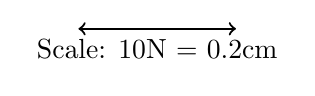
\begin{tikzpicture}[scale=0.2]
        \draw[thick, <->] (-10cm,0) -- node[below] {Scale: 10N = 0.2cm} ++(10cm,0);
    \end{tikzpicture}


    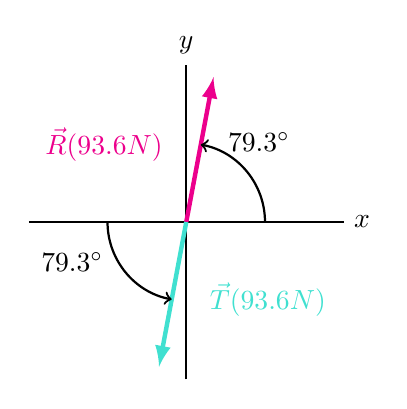
\begin{tikzpicture}[scale=0.2]

        \coordinate (O) at (0,0);

        \draw[thick, -] (-10cm,0cm) coordinate(leftx) -- (10cm,0cm) coordinate(rightx) node[right,fill=white]{$x$};

        \draw[thick, -] (0cm,-10cm) coordinate(bottomy) -- (0cm,10cm) coordinate(topy) node[above,fill=white] {$y$};

        \draw[magenta, ultra thick, -latex] (0cm,0cm) -- (1.73cm, 9.2cm) coordinate(R) node[shift={(-0.5, -0.5)}, pos=1,anchor=north east, magenta]{$\vec{R} (93.6 N)$};

        \pic [draw, ->, "$79.3^\circ$", angle eccentricity=1.2, anchor=south, thick, angle radius=1cm] {angle = rightx--O--R};

        \draw[Turquoise, ultra thick, -latex] (0cm,0cm) -- (-1.73cm, -9.2cm) coordinate(R) node[shift={(0.5, 0.5)}, pos=1, anchor=south west, Turquoise]{$\vec{T} (93.6 N)$};

        \pic [draw, ->, "$79.3^\circ$", angle eccentricity=1.2, anchor=south east, thick, angle radius=1cm] {angle = leftx--O--R};

    \end{tikzpicture}
\end{figure}

In this case, vector $\vec{T}$ is acting opposite of the resultant vector $\vec{R}$, such that:
\[\vec{T} = -\vec{R}\]

To demonstrate this using the component method, we can simply utilize the methods in Table 1, but add the fourth vector $\vec{T}$ whose components are the opposite of the resultant vector $\vec{R}$.

\begin{figure}[H]
    \centering
    \begin{tabular}{ |p{3cm}|p{3cm}|p{3cm}| }
        \hline
        \multicolumn{3}{|c|}{Table 2: The resultant vector after adding vector $\vec{T}$}              \\
        \hline
        Vector $\vec{V}$                              & $\vec{V_x}$ (N) & $\vec{V_y}$ (N) \\
        \hline
        $\vec{A}$                                     & 86.6            & 50.0            \\
        $\vec{B}$                                     & -40             & 69.3            \\
        $\vec{C}$                                     & -29.3           & -27.3           \\
        $\vec{T}$                                     & -17.3           & -92.0           \\
        \hline
        $\vec{A}$ + $\vec{B}$ + $\vec{C}$ + $\vec{T}$ & 0.0             & 0.0             \\
        \hline
    \end{tabular}
\end{figure}

In this case, it can be said that the particle is in translational equalibrium because the net force acting on the particle is 0 with the inclusion of the 4th vector $\vec{T}$.
\section{Conclusion}
In the beginning, we set out to determine whether or not we could arrive at similar physical quantities using two different methods of vector addition. The visual method, known as the head to tail method, involved rearanging the vectors in a manner such that a new vector could be drawn from the tail of the first vector, to the head last vector on some x-y coordinate plane. The second method involved summing the projections that each vector made on the respective x and y axis and using trigonometry to recover the magnitude and angle of the new components.

I hypothesized that both methods would yield similar results but the head to tail method would be slightly less accurate. There turned out to be a margin of error of about 1.3N in the magnitude and $1.3^\circ$ in the direction using the head to tail method which is consistent with my hypothesis that the method would be less accurate. However, despite this margin of error, both methods did yield very similar results. This leads me to believe that our data was conclusive in determining the validity and accuracy of the methods discussed in the lab.

\end{document}
